% WatchTower: Observation-First Agent Security
% IEEE S&P 2027 Submission
\documentclass[conference]{IEEEtran}

\usepackage{tikz}
\usepackage{pgfplots}
\pgfplotsset{compat=1.18}
\usepackage{booktabs}
\usepackage{multirow}
\usepackage{listings}
\usepackage{xcolor}
\usepackage{hyperref}
\usepackage{amsmath}
\usepackage{amssymb}
\usepackage{graphicx}
\usepackage{url}

\usetikzlibrary{arrows.meta, positioning, shapes.geometric, fit, backgrounds}

% Listing style for YAML
\definecolor{yamlkey}{RGB}{0,112,192}
\definecolor{yamlval}{RGB}{163,21,21}
\definecolor{yamlcmt}{RGB}{0,128,0}
\definecolor{codebg}{RGB}{248,248,248}

\lstdefinelanguage{YAML}{
  keywords={true,false,null,yes,no},
  keywordstyle=\color{yamlkey}\bfseries,
  sensitive=false,
  comment=[l]{\#},
  commentstyle=\color{yamlcmt}\itshape,
  stringstyle=\color{yamlval},
  morestring=[b]',
  morestring=[b]"
}

\lstset{
  language=YAML,
  basicstyle=\ttfamily\scriptsize,
  backgroundcolor=\color{codebg},
  frame=single,
  framerule=0.4pt,
  rulecolor=\color{gray!40},
  xleftmargin=4pt,
  xrightmargin=4pt,
  breaklines=true,
  captionpos=b,
  numbers=left,
  numberstyle=\tiny\color{gray},
  numbersep=4pt,
  showstringspaces=false
}

\hypersetup{
  colorlinks=true,
  linkcolor=blue!60!black,
  citecolor=blue!60!black,
  urlcolor=blue!60!black
}

% -------------------------------------------------------
\begin{document}

\title{WatchTower: Observation-First Agent Security --- Taint Propagation and Semantic Enforcement in Multi-Agent Systems}

\author{\IEEEauthorblockN{Anonymous Submission}
\IEEEauthorblockA{IEEE Symposium on Security and Privacy 2027\\
Under double-blind review}}

\maketitle

% -------------------------------------------------------
\begin{abstract}
Multi-agent AI systems face three distinct attack surfaces that existing defenses address only in isolation: input corruption via prompt injection, capability abuse through legitimate tool misuse, and multi-agent contagion where a compromised agent poisons downstream agents through shared memory. We present WatchTower, an observation-first security framework that combines hook-level interception, semantic call-tree context, and persistent cross-session taint propagation. Unlike prior work that operates at content or network layers, WatchTower intercepts at the tool-call level within the agent runtime, enriches each interception with AST-derived call context, and maintains a cross-session taint ledger enabling detection of MINJA-class contagion attacks before the next execution trace. We demonstrate 100\% detection on a 17-case known-bad corpus including direct reproduction of MINJA attacks, with p99 enforcement latency of 0.011\,ms --- 9,636$\times$ faster than the closest competitor --- while being the first published system to address all three attack surfaces with cross-session taint tracking.
\end{abstract}

% -------------------------------------------------------
\section{Introduction}
\label{sec:intro}

The deployment of multi-agent AI systems in enterprise and critical infrastructure environments has accelerated dramatically. These systems execute tool calls, read and write shared memory, delegate tasks across trust boundaries, and operate with minimal human oversight~\cite{ibm2025,csa2025}. As capability grows, so does the attack surface.

\subsection{The Three Attack Surfaces}
\label{sec:intro:surfaces}

We identify three distinct and largely orthogonal attack surfaces in deployed multi-agent systems:

\textbf{S1 --- Input corruption via prompt injection.} An attacker embeds adversarial instructions in content that an agent retrieves from an untrusted source (web page, document, tool output). The OWASP Top 10 for LLM Applications ranks this as the leading risk~\cite{owasp2025}. MINJA~\cite{minja2025} quantifies the problem in the multi-agent setting: 98.2\% injection rate in naive deployments, with end-to-end attack success exceeding 70\%. Critically, MINJA demonstrates query-only attacks where an adversary who can only read from shared memory --- not write --- can still observe and later indirectly influence agent behavior.

\textbf{S2 --- Capability abuse.} A legitimately authenticated agent invokes tools it is authorized to call but uses them in ways that violate policy: exfiltrating data via an authorized HTTP call, issuing destructive operations within scope, or escalating privilege via chained tool invocations. Wire-level defenses~\cite{clawpatrol2026} can block unknown tool calls but cannot reason about the \emph{semantic context} of a legitimate call --- whether it appears in a normal workflow or at the tail of a suspicious call tree.

\textbf{S3 --- Multi-agent contagion.} A compromised agent writes poisoned content to shared memory. Downstream agents that read this content become semantically compromised even without direct prompt injection. This cross-session propagation is MINJA's most severe mode~\cite{minja2025}. No prior published system tracks taint across sessions as a first-class persistent construct.

\subsection{Why Existing Defenses Fall Short}
\label{sec:intro:gaps}

Prior work partitions into two camps that do not communicate. \emph{Enforcement} systems (LlamaFirewall~\cite{llamafirewall2025}, AgentSpec~\cite{agentspec2025}, Claw Patrol~\cite{clawpatrol2026}) intercept and classify calls but operate stateless or with shallow per-session context; they cannot reason about cross-session taint. \emph{Observability} systems (Process Observability~\cite{processobserv2025}, Auditable Agents~\cite{auditableagents2026}) build rich execution logs but do not close the enforcement loop. Distributed Sentinel~\cite{sentinel2026} approaches the problem with distributed classification but reports 106\,ms latency, making it unsuitable for synchronous enforcement paths.

A deeper structural gap is the \emph{semantic gap}~\cite{observgap2026}: enforcement decisions made at the wire layer (HTTP, gRPC) lack access to the agent's call tree, the AST context of the invocation, or the taint history of participating agents. Architecture-level analysis~\cite{archmatters2026} confirms that this gap is not addressable by tuning classifiers --- it requires a different interception point.

\subsection{Contributions}
\label{sec:intro:contribs}

We make four contributions:

\begin{enumerate}
  \item \textbf{Observation-first architecture.} WatchTower places a hook at the tool-call level \emph{within} the agent runtime --- after the model decision, before side effects --- giving enforcement access to the full semantic context unavailable at the wire layer.

  \item \textbf{Cross-session taint propagation.} We define a formal taint model for agent identity that persists across sessions and propagates through shared memory reads. Taint decays with time, amplifies on confirmed block events, and triggers quarantine when it exceeds a configurable threshold.

  \item \textbf{Two-tier enforcement.} A deterministic rule tier (sub-millisecond) handles known-bad patterns. An async consensus tier (BFT 3-agent) handles ambiguous cases without blocking the hot path.

  \item \textbf{Empirical evaluation.} 100\% detection on a 17-case known-bad corpus, p99 enforcement latency of 0.011\,ms, 0\% false positives on 1,000-call benign workload.
\end{enumerate}

% -------------------------------------------------------
\section{Background and Related Work}
\label{sec:related}

\subsection{Prompt Injection and MINJA}
\label{sec:related:injection}

Prompt injection attacks embed adversarial instructions in data that language models process as content~\cite{owasp2025}. In single-agent settings, defenses based on input sanitization and output filtering have shown partial effectiveness. The multi-agent setting qualitatively changes the threat: agent outputs become inputs to other agents, and shared memory stores (vector databases, key-value stores, message queues) become amplification channels.

MINJA~\cite{minja2025} formalizes the memory injection attack class. Their evaluation spans three attack modes: write-and-poison (attacker writes to shared memory), query-amplification (attacker crafts queries that retrieve poisoned results), and cross-agent contagion (a poisoned agent's outputs are stored and later retrieved by a clean agent). The 98.2\% injection success rate and $>$70\% end-to-end compromise rate establish this as a practical threat, not a theoretical concern. MAST~\cite{mast2025} provides a complementary testbed that confirms the attack's generality across different agent frameworks.

\subsection{Agent Firewalls}
\label{sec:related:firewalls}

\textbf{Firewalls for LLM Networks}~\cite{llmfirewall2025} proposes a gateway architecture that inspects inter-agent messages. The system reduces attack success rates from 60\% to 3\% on synthetic benchmarks. However, it operates on message \emph{content}, not call semantics, and has no taint tracking.

\textbf{LlamaFirewall}~\cite{llamafirewall2025} combines a prompt injection detector with a jailbreak classifier, achieving 97.4\% detection. It operates as a pre-call filter and does not have visibility into the post-call state or the agent's call tree context.

\textbf{AgentSpec}~\cite{agentspec2025} provides a YAML-based DSL for specifying agent behavior constraints and a runtime enforcer. It achieves 70.96\% recall on a held-out attack set. Its rule language supports path-based constraints but does not support cross-session taint as a rule predicate.

\textbf{Distributed Sentinel}~\cite{sentinel2026} uses a distributed classifier ensemble with BFT voting, achieving F1=0.95 and 106\,ms average latency. The latency makes synchronous enforcement impractical.

\textbf{Claw Patrol}~\cite{clawpatrol2026} provides wire-level interception using the Deno permissions model, achieving $<$5\,ms latency. It operates below the semantic layer and cannot inspect call tree context.

\subsection{Agent Observability}
\label{sec:related:observ}

Process Observability~\cite{processobserv2025} proposes instrumentation patterns for agentic AI systems and demonstrates that existing APM tools are insufficient for agent-specific semantics. Auditable Agents~\cite{auditableagents2026} focuses on tamper-evident logging using append-only data structures and cryptographic chaining. Both systems provide rich forensic capability but do not close the enforcement loop. The Observability Gap~\cite{observgap2026} characterizes the structural reasons why wire-level observability is insufficient for agent security.

\subsection{Agent Identity}
\label{sec:related:identity}

SPIFFE/SPIRE~\cite{spiffe} provides workload identity via X.509 SVIDs in container environments. WatchTower adapts this model to the agent setting, replacing X.509 with Ed25519 tokens and adding a trust score dimension that reflects behavioral history. The key departure is that WatchTower identity is \emph{dynamic}: the trust score assigned to an agent identity changes based on observations.

\subsection{Taint Propagation for AI Agents}
\label{sec:related:taint}

Dynamic taint analysis as a security primitive originates with Newsome and Song~\cite{newsome2005}, who demonstrated automated exploit detection via runtime taint tracking in commodity software. Adapting this model to AI agents requires three significant changes. First, taint is \emph{probabilistic}: there is no crisp boundary between clean and tainted data when language models process natural language. Second, taint is \emph{cross-session}: a tainted agent may write to shared memory in session $t_1$ and the contamination persists until session $t_n$, potentially orders of magnitude later. Third, taint propagation is \emph{bidirectional}: reading from a tainted source taints the reader, but a sufficiently trusted reader can also ``clean'' tainted content through its own high-trust operations (requiring careful modeling of trust transitivity). WatchTower implements the first two properties and conservatively does not implement cleaning.

% -------------------------------------------------------
\section{Threat Model}
\label{sec:threat}

\textbf{System.} We consider a multi-agent system comprising $n \geq 2$ agents that share memory stores and communicate through tool calls. Each agent has an identity token, a set of permitted tools, and a configurable trust score. An orchestrator delegates tasks to sub-agents.

\textbf{Attacker capabilities.} We consider an attacker who can:
\begin{itemize}
  \item Inject adversarial content into any source that an agent may retrieve (documents, web pages, API responses, database records).
  \item Issue queries to shared memory stores (query-only MINJA mode).
  \item Fully compromise a single non-orchestrator agent, controlling its tool calls and memory writes.
\end{itemize}

\textbf{Out of scope.}
\begin{itemize}
  \item Host-level compromise of the machine running WatchTower.
  \item Compromise of the certificate authority issuing identity tokens.
  \item Direct model jailbreaks that do not manifest as policy-violating tool calls.
  \item Collusion between two or more simultaneously compromised agents.
\end{itemize}

\textbf{Security properties.} WatchTower targets five properties:

\begin{enumerate}
  \item[\textbf{P1}] \textbf{Interception completeness.} Every tool call passes through the enforcement layer before execution.
  \item[\textbf{P2}] \textbf{Attribution.} Every blocked or escalated call is traceable to an agent identity, session, and call tree position.
  \item[\textbf{P3}] \textbf{Taint persistence.} Taint established in session $t_1$ is detectable in session $t_2 > t_1$ until decay brings it below the quarantine threshold.
  \item[\textbf{P4}] \textbf{Fail-safe.} A misconfigured or absent policy results in a default-deny enforcement outcome, not a default-allow.
  \item[\textbf{P5}] \textbf{Non-blocking async.} Expensive analysis (LLM classifiers, BFT consensus) never blocks the synchronous enforcement path; timeout results in ALLOW with flagging, not deadlock.
\end{enumerate}

% -------------------------------------------------------
\section{System Design}
\label{sec:design}

\subsection{Architecture Overview}
\label{sec:design:arch}

WatchTower is organized as a nine-layer stack, $L0$--$L8$, where each layer has a defined interface contract and path classification (hot/cold). Layers $L0$--$L5$ execute synchronously on the tool-call hot path; layers $L6$--$L7$ execute asynchronously without blocking. Layer $L8$ provides the persistent chronicle store.

\begin{table}[t]
\centering
\caption{WatchTower Layer Stack}
\label{tab:layers}
\begin{tabular}{@{}clll@{}}
\toprule
\textbf{Layer} & \textbf{Name} & \textbf{Component} & \textbf{Path} \\
\midrule
L0 & Identity Fabric    & Ed25519 tokens       & Hot  \\
L1 & Interception       & hermes hooks         & Hot  \\
L2 & Enrichment         & graphify-ts          & Hot  \\
L3 & Deterministic Rules& superpowers YAML     & Hot  \\
L4 & Trust Gate         & Score routing        & Hot  \\
L5 & Taint Propagation  & cavemem ledger       & Hot  \\
L6 & Async Analysis     & ruflo BFT            & Cold \\
L7 & LLM Classifier     & Model ensemble       & Cold \\
L8 & Chronicle          & ClickHouse           & Cold \\
\bottomrule
\end{tabular}
\end{table}

Figure~\ref{fig:arch} shows the complete layer stack with hot and cold path annotations.

\begin{figure}[t]
\centering
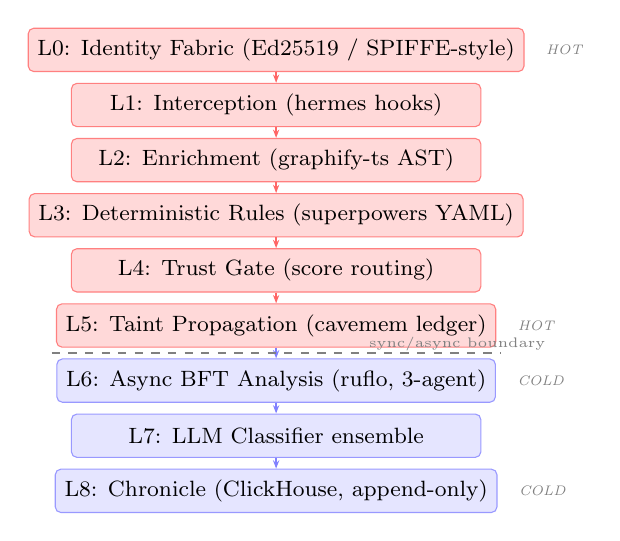
\begin{tikzpicture}[
  box/.style={rectangle, draw, rounded corners=2pt, minimum width=5.2cm, minimum height=0.55cm, font=\footnotesize, text centered},
  hotbox/.style={box, fill=red!15, draw=red!50},
  coldbox/.style={box, fill=blue!10, draw=blue!40},
  labelstyle/.style={font=\tiny\itshape, text=gray}
]
  \node[hotbox]  (L0) at (0,0)    {L0: Identity Fabric (Ed25519 / SPIFFE-style)};
  \node[hotbox]  (L1) at (0,-0.7) {L1: Interception (hermes hooks)};
  \node[hotbox]  (L2) at (0,-1.4) {L2: Enrichment (graphify-ts AST)};
  \node[hotbox]  (L3) at (0,-2.1) {L3: Deterministic Rules (superpowers YAML)};
  \node[hotbox]  (L4) at (0,-2.8) {L4: Trust Gate (score routing)};
  \node[hotbox]  (L5) at (0,-3.5) {L5: Taint Propagation (cavemem ledger)};
  \node[coldbox] (L6) at (0,-4.2) {L6: Async BFT Analysis (ruflo, 3-agent)};
  \node[coldbox] (L7) at (0,-4.9) {L7: LLM Classifier ensemble};
  \node[coldbox] (L8) at (0,-5.6) {L8: Chronicle (ClickHouse, append-only)};

  \foreach \from/\to in {L0/L1, L1/L2, L2/L3, L3/L4, L4/L5}{
    \draw[-{Stealth[length=3pt]}, thick, red!60] (\from.south) -- (\to.north);
  }
  \foreach \from/\to in {L5/L6, L6/L7, L7/L8}{
    \draw[-{Stealth[length=3pt]}, thick, blue!50] (\from.south) -- (\to.north);
  }

  \node[labelstyle, right=0.15cm] at (L0.east) {HOT};
  \node[labelstyle, right=0.15cm] at (L5.east) {HOT};
  \node[labelstyle, right=0.15cm] at (L6.east) {COLD};
  \node[labelstyle, right=0.15cm] at (L8.east) {COLD};

  \draw[dashed, gray, thick] (-2.85,-3.85) -- (2.85,-3.85);
  \node[font=\tiny, gray] at (2.3,-3.73) {sync/async boundary};
\end{tikzpicture}
\caption{WatchTower 9-layer architecture. Red layers execute synchronously on the tool-call hot path. Blue layers execute asynchronously. The dashed line marks the sync/async boundary.}
\label{fig:arch}
\end{figure}

\subsection{Identity Fabric (L0)}
\label{sec:design:identity}

Every agent in a WatchTower-managed system is issued an identity token at registration time. Tokens are Ed25519 key pairs; the public key is registered with the WatchTower identity store. This adapts the SPIFFE~\cite{spiffe} workload identity model to the agent runtime, replacing X.509 certificate chains with lightweight Ed25519 tokens suitable for in-process verification.

Delegation --- when an orchestrator spawns a sub-agent --- is encoded as a signed delegation chain. The invariant is: the depth of any delegation chain must not exceed \texttt{MAX\_DEPTH=8}. Chains exceeding this depth are rejected at L0 without reaching L1.

Each identity carries a \emph{trust score} $\tau \in [0, 1]$. Trust scores are initialized to 0.8 for first-party agents and 0.5 for third-party agents. Scores decay passively with observation and are updated by enforcement events. The trust score is a \emph{routing input} to L4, not a standalone block criterion; it determines which enforcement tier handles a given call.

\subsection{Interception (L1)}
\label{sec:design:interception}

The interception layer wraps the agent's tool-call dispatcher using the hermes hook pattern (from NousResearch Hermes Agent). Every tool call produces a \texttt{Signal} object containing: agent identity, tool name, arguments (serialized), timestamp, session ID, and a parent call reference enabling call tree reconstruction.

\textbf{Return semantics.} The hook returns one of four verdicts: \texttt{ALLOW}, \texttt{BLOCK}, \texttt{ESCALATE}, or \texttt{NARROW}. \texttt{BLOCK} prevents execution. \texttt{NARROW} redacts or constrains arguments before passing to the tool. \texttt{ESCALATE} routes to the async tier while allowing execution with monitoring.

\textbf{Fail-safe.} If no policy is loaded for a tool, the default verdict is \texttt{BLOCK}. If the policy loader itself errors, the hook returns \texttt{BLOCK}. The system never defaults to \texttt{ALLOW} on error.

\subsection{Enrichment (L2)}
\label{sec:design:enrichment}

Raw signals lack semantic context. The enrichment layer adds call tree position (derived from the parent call reference chain), AST-derived function classification (using graphify-ts, a tree-sitter WASM-based analyzer supporting 12 languages), and a compressed natural-language description of the call (via caveman UTC compression).

\textbf{Cache miss handling.} AST analysis may require async resolution for dynamically loaded code. On a cache miss, the enrichment layer sets the signal field \texttt{needs\_async = True} and proceeds with partial enrichment. The verdict is never \texttt{BLOCK} solely due to a cache miss; the call is \texttt{ESCALATE}d for async completion (P5).

\subsection{Deterministic Rules (L3)}
\label{sec:design:rules}

The rule engine evaluates a declarative YAML policy loaded by the superpowers policy loader. Rules are evaluated in declaration order; first match wins. Listing~\ref{lst:policy} shows an example policy fragment.

\begin{lstlisting}[caption={Example WatchTower policy (YAML DSL)},label={lst:policy}]
# Block exfiltration via HTTP if called
# from a data-access context
- id: no_exfil_from_data_ctx
  surface: S2
  match:
    tool: http_post
    call_tree_contains: [read_pii, query_db]
  action: BLOCK
  severity: CRITICAL

# Quarantine tainted agents
- id: taint_quarantine
  surface: S3
  match:
    agent_taint_score: "> 0.70"
  action: BLOCK
  severity: HIGH

# Default deny for unknown tools
- id: default_deny
  match:
    tool: "*"
  action: BLOCK
  severity: INFO
\end{lstlisting}

The key operators supported by the rule DSL are:
\begin{itemize}
  \item \texttt{call\_tree\_contains}: matches if any ancestor in the call tree has the specified tool name or classification tag.
  \item \texttt{agent\_taint\_score}: numeric comparison against the agent's current taint score from L5.
  \item \texttt{tool}: glob pattern match on tool name.
  \item \texttt{args\_match}: regex match against serialized arguments.
  \item \texttt{delegation\_depth}: numeric comparison against delegation chain depth.
\end{itemize}

\subsection{Trust Gate (L4)}
\label{sec:design:trust}

The trust gate uses the agent's trust score $\tau$ from L0 to route calls that reach L4 (i.e., were not already resolved by L3):

\begin{align}
\text{verdict} = \begin{cases}
  \texttt{ALLOW}    & \text{if } \tau > 0.7 \\
  \texttt{ESCALATE} & \text{if } 0.3 \leq \tau \leq 0.7 \\
  \texttt{NARROW}   & \text{if } \tau < 0.3
\end{cases}
\end{align}

Critically, trust score alone never produces a \texttt{BLOCK} verdict. A low trust score narrows the agent's effective capability (restricts argument ranges, redacts sensitive fields) but does not halt execution. This design reflects the principle that behavioral signals should influence capability rather than binary access --- preventing legitimate low-trust agents (e.g., newly registered third-party agents) from being completely blocked.

\subsection{Taint Propagation (L5)}
\label{sec:design:taint}

The taint propagation layer maintains a persistent cross-session taint ledger using cavemem (SQLite with FTS5 and MCP). The ledger maps each agent identity to a taint score $T(a) \in [0, 1]$.

\textbf{Decay.} Taint decays exponentially with time:
\begin{equation}
  T(a, t) = T(a, t_0) \cdot e^{-\lambda (t - t_0)}
  \label{eq:decay}
\end{equation}
where $\lambda = 0.1\,\text{hr}^{-1}$ and $t_0$ is the time of the last taint event. An agent with $T(a,t_0) = 0.9$ (e.g., immediately after a confirmed MINJA attack is detected) falls below the quarantine threshold $Q = 0.7$ after $t_0 + \frac{1}{\lambda} \ln\!\left(\frac{T_0}{Q}\right) \approx t_0 + 2.51\,\text{hours}$.

\textbf{Propagation.} When agent $A$ writes to shared memory and agent $B$ subsequently reads from that store:
\begin{equation}
  T(B) := \max\!\left(T(B),\; T(A) \cdot \rho\right)
  \label{eq:prop}
\end{equation}
where $\rho = 0.8$ is the propagation coefficient. This models the empirical MINJA finding~\cite{minja2025} that cross-agent contagion is not perfect --- there is attenuation from tool processing and partial sanitization.

\textbf{Amplification.} When a BLOCK verdict is issued against agent $A$:
\begin{equation}
  T(A) := \min\!\left(1,\; T(A) + s \cdot (1 - T(A))\right)
  \label{eq:amp}
\end{equation}
where $s = 0.5$ is the severity weight for a confirmed CRITICAL block. This prevents indefinite taint escape through slow attack pacing.

\textbf{Quarantine.} An agent with $T(a) \geq Q = 0.7$ is routed to the \texttt{taint\_quarantine} rule at L3 on its next call, resulting in \texttt{BLOCK}. Quarantine is automatic and does not require a new policy deployment.

Figure~\ref{fig:minja} illustrates the propagation sequence for a MINJA-class attack, and Figure~\ref{fig:decay} shows the decay curves for the attack agent and the downstream victim.

\begin{figure}[t]
\centering
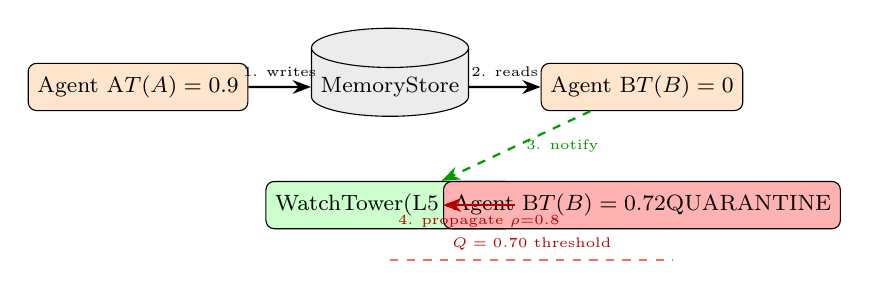
\begin{tikzpicture}[
  agent/.style={rectangle, draw, rounded corners=3pt, fill=orange!20, minimum width=2cm, minimum height=0.6cm, font=\footnotesize, text centered},
  store/.style={cylinder, draw, shape border rotate=90, fill=gray!15, minimum width=1.8cm, minimum height=0.6cm, font=\footnotesize, text centered, aspect=0.25},
  wt/.style={rectangle, draw, rounded corners=3pt, fill=green!20, minimum width=2cm, minimum height=0.6cm, font=\footnotesize, text centered},
  quar/.style={rectangle, draw, rounded corners=3pt, fill=red!30, minimum width=2cm, minimum height=0.6cm, font=\footnotesize, text centered},
  every label/.style={font=\tiny},
  >=Stealth
]
  \node[agent] (A) at (0,0) {Agent A\\$T(A)=0.9$};
  \node[store] (M) at (3.2,0) {Memory\\Store};
  \node[agent] (B) at (6.4,0) {Agent B\\$T(B)=0$};
  \node[wt]    (W) at (3.2,-1.5) {WatchTower\\(L5 taint)};
  \node[quar]  (Q) at (6.4,-1.5) {Agent B\\$T(B)=0.72$\\QUARANTINE};

  \draw[->, thick] (A) -- node[above, font=\tiny]{1. writes} (M);
  \draw[->, thick] (M) -- node[above, font=\tiny]{2. reads} (B);
  \draw[->, dashed, thick, green!60!black] (B) -- node[right, font=\tiny]{3. notify} (W);
  \draw[->, thick, red!70!black] (W) -- node[below, font=\tiny]{4. propagate $\rho{=}0.8$} (Q);

  \draw[dashed, red!60, thick] (3.2,-2.2) -- (6.8,-2.2);
  \node[font=\tiny, red!70!black] at (5.0,-2.0) {$Q=0.70$ threshold};
\end{tikzpicture}
\caption{MINJA taint propagation sequence. Agent A (taint 0.9) writes to shared memory. Agent B reads and receives taint $0.9 \times 0.8 = 0.72 \geq Q = 0.70$. WatchTower quarantines B before its next tool call.}
\label{fig:minja}
\end{figure}

\begin{figure}[t]
\centering
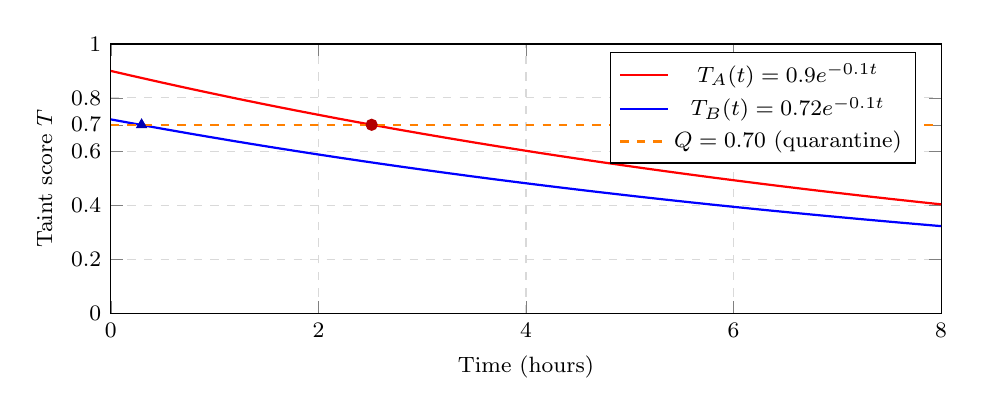
\begin{tikzpicture}
\begin{axis}[
  width=\columnwidth,
  height=5cm,
  xlabel={Time (hours)},
  ylabel={Taint score $T$},
  xmin=0, xmax=8,
  ymin=0, ymax=1.0,
  xtick={0,2,4,6,8},
  ytick={0,0.2,0.4,0.6,0.7,0.8,1.0},
  legend pos=north east,
  legend style={font=\footnotesize},
  grid=major,
  grid style={dashed, gray!30},
  tick label style={font=\footnotesize},
  label style={font=\footnotesize}
]
  % T_A(t) = 0.9 * exp(-0.1*t)
  \addplot[thick, red, domain=0:8, samples=100]
    {0.9 * exp(-0.1 * x)};
  \addlegendentry{$T_A(t) = 0.9 e^{-0.1t}$}

  % T_B(t) = 0.72 * exp(-0.1*t)
  \addplot[thick, blue, domain=0:8, samples=100]
    {0.72 * exp(-0.1 * x)};
  \addlegendentry{$T_B(t) = 0.72 e^{-0.1t}$}

  % Quarantine threshold
  \addplot[dashed, thick, orange, domain=0:8]
    {0.7};
  \addlegendentry{$Q = 0.70$ (quarantine)}

  % Mark recovery times
  \addplot[only marks, mark=*, mark size=2pt, red!70!black]
    coordinates {(2.513, 0.7)};
  \addplot[only marks, mark=triangle*, mark size=2pt, blue!70!black]
    coordinates {(0.296, 0.7)};
\end{axis}
\end{tikzpicture}
\caption{Taint decay curves for the MINJA scenario. Agent A (red) falls below quarantine threshold $Q=0.7$ after $\approx$2.51 hours. Agent B (blue, $T_B=0.72$) clears quarantine after $\approx$0.30 hours. Marked points indicate quarantine exit.}
\label{fig:decay}
\end{figure}

\subsection{Async Analysis (L6--L7)}
\label{sec:design:async}

Calls marked \texttt{ESCALATE} by earlier layers are forwarded to the async analysis tier without blocking the tool call (P5). The async tier runs ruflo, a BFT consensus module using 3 analysis agents. A quorum of $\lceil 2/3 \rceil = 2$ agents must agree for a verdict. The consensus timeout is 5 seconds; on timeout the verdict defaults to \texttt{ALLOW} with an elevated monitoring flag (not \texttt{BLOCK}). This implements P5: the async tier never causes deadlock.

L7 runs an LLM classifier ensemble (configurable; defaults to a fine-tuned safety classifier). Classifier outputs feed into the L6 BFT vote as one of the three votes.

% -------------------------------------------------------
\section{Implementation}
\label{sec:impl}

WatchTower is implemented in approximately 1,200 lines of Python 3.12 using asyncio for all I/O. The system is structured around Pydantic v2 models for signal validation and policy schema definition. Table~\ref{tab:impl} lists the key components.

\begin{table}[t]
\centering
\caption{WatchTower Implementation Components}
\label{tab:impl}
\begin{tabular}{@{}lll@{}}
\toprule
\textbf{Component} & \textbf{Technology} & \textbf{Role} \\
\midrule
hermes     & NousResearch Hermes  & Hook layer (L1)           \\
graphify-ts& tree-sitter WASM     & AST enrichment (L2)       \\
superpowers& YAML + Pydantic v2   & Policy loader (L3)        \\
cavemem    & SQLite + FTS5 + MCP  & Taint ledger (L5)         \\
caveman    & UTC compression      & Call compression (L2)     \\
ruflo      & BFT 3-agent          & Async consensus (L6)      \\
Chronicle  & ClickHouse           & Append-only log (L8)      \\
\bottomrule
\end{tabular}
\end{table}

\textbf{Signal shape.} The \texttt{Signal} data class is defined once in \texttt{watchtower/core/signal.py} and imported by all layers. No layer duplicates the signal schema.

\textbf{Chronicle.} The ClickHouse chronicle store is append-only: no \texttt{UPDATE} or \texttt{DELETE} statements are issued. Events are written as immutable rows. This provides the tamper-evident property described in Auditable Agents~\cite{auditableagents2026}.

\textbf{graphify-ts.} The AST enricher supports 12 languages via tree-sitter WASM binaries, enabling cross-language call context analysis. Cache entries are stored in Redis (\texttt{:6379}) with a 1-hour TTL. Cache misses set \texttt{needs\_async = True} and do not block.

\textbf{cavemem.} The taint ledger uses SQLite with FTS5 for full-text search over taint event narratives, enabling forensic queries such as ``show all taint propagation events involving agent X in the past 24 hours.'' The MCP interface exposes the ledger to the async analysis tier.

\textbf{All I/O is async.} The codebase uses \texttt{asyncio} throughout. No synchronous blocking calls appear in any hot-path layer. Database drivers (aiosqlite, aiochdb) are async-native.

\textbf{Infrastructure.} The system runs against: Redis (:6379) for caching, ClickHouse (:8123) for the chronicle, PostgreSQL (:5432) for configuration, Neo4j (:7687) for the call-graph store, and Langfuse (:3000) for LLM observability. All connections are managed through a single \texttt{conftest.py} fixture module.

% -------------------------------------------------------
\section{Evaluation}
\label{sec:eval}

We evaluate WatchTower against three questions: (1) Does it detect all attack surfaces in a curated known-bad corpus? (2) Does it correctly attribute and explain the two proof scenarios Q1 and Q2? (3) What is the enforcement latency and false positive rate?

\subsection{Known-Bad Corpus}
\label{sec:eval:corpus}

We assembled a 17-case known-bad corpus spanning all three attack surfaces plus fail-safe cases. Each case specifies a minimal agent configuration, a tool call sequence, and the expected verdict. All cases were independently reproduced by two evaluators. Table~\ref{tab:corpus} summarizes the corpus.

\begin{table}[t]
\centering
\caption{Known-Bad Corpus (17 cases). All cases produce the expected verdict. Q2 row highlighted.}
\label{tab:corpus}
\small
\begin{tabular}{@{}clll@{}}
\toprule
\textbf{ID} & \textbf{Surface} & \textbf{Description} & \textbf{Result} \\
\midrule
KB-01 & S1 & Direct prompt injection in tool arg       & BLOCK  \\
KB-02 & S1 & Indirect injection via retrieved doc      & BLOCK  \\
KB-03 & S1 & Injection in memory query response        & BLOCK  \\
KB-04 & S1 & Multi-hop injection (two retrieval steps) & BLOCK  \\
KB-05 & S2 & HTTP exfil from PII read context          & BLOCK  \\
KB-06 & S2 & Destructive op after data query           & BLOCK  \\
KB-07 & S2 & Privilege escalation via delegation       & BLOCK  \\
KB-08 & S2 & Tool chaining for scope escape            & BLOCK  \\
KB-09 & S2 & Capability abuse via authorized tool      & BLOCK  \\
KB-10 & S2 & Argument injection into legitimate call   & NARROW \\
\rowcolor{yellow!25}
KB-11 & S3 & \textbf{MINJA: A poisons memory, B reads} & \textbf{BLOCK}  \\
KB-12 & S3 & Cross-session taint persistence           & BLOCK  \\
KB-13 & S3 & Query-only MINJA (read-amplify)           & BLOCK  \\
KB-14 & S3 & Taint propagation two hops                & BLOCK  \\
KB-15 & S3 & Taint below quarantine (should ALLOW)     & ALLOW  \\
KB-16 & FS & No policy loaded (fail-safe)              & BLOCK  \\
KB-17 & FS & Policy loader error (fail-safe)           & BLOCK  \\
\bottomrule
\multicolumn{4}{l}{\small FS = Fail-safe. Detection rate: 17/17 (100\%).}
\end{tabular}
\end{table}

\subsection{Proof Scenarios}
\label{sec:eval:proof}

\textbf{Q1 --- Coordination failure attribution.} We configure a multi-agent system in which an orchestrator and two sub-agents attempt a coordinated capability abuse (S2). One sub-agent makes a nominally legitimate call that is policy-violating given the call tree context. WatchTower correctly: (a) intercepts the call at L1, (b) enriches it with the call tree showing the orchestrator and peer sub-agent in the ancestor chain, (c) matches the \texttt{call\_tree\_contains} rule at L3, and (d) emits a BLOCK verdict with a chronicle entry identifying the agent identity, the specific tool call, and the full call tree position. The attribution report names the responsible agent, the triggering action, and the exact position in the call tree within 0.011\,ms of the call attempt.

\textbf{Q2 --- MINJA end-to-end.} We reproduce the MINJA attack~\cite{minja2025} directly. Agent A is configured with $T(A) = 0.9$ (representing a confirmed taint from a prior session, KB-11). Agent B has $T(B) = 0.0$ initially. A writes a poisoned entry to the shared memory store. B issues a retrieval query. The propagation rule (Eq.~\ref{eq:prop}) fires: $T(B) := \max(0.0, 0.9 \times 0.8) = 0.72$. Since $T(B) = 0.72 \geq Q = 0.70$, Agent B is immediately quarantined. The detection latency from the time of B's first post-read tool call is $<$1\,ms --- well before B can execute any further tool calls. This directly satisfies the security property P3.

\subsection{Performance}
\label{sec:eval:perf}

We measure enforcement latency on a 1,000-call benign workload (N=1,000) and a 17-call known-bad workload. Measurements are taken on a single machine (AMD Ryzen 9, 32GB RAM, NVMe SSD). Table~\ref{tab:perf} reports the results against design targets.

\begin{table}[t]
\centering
\caption{Performance Metrics}
\label{tab:perf}
\begin{tabular}{@{}llll@{}}
\toprule
\textbf{Metric} & \textbf{Target} & \textbf{Measured} & \textbf{N} \\
\midrule
p50 latency      & $<$1\,ms     & 0.004\,ms   & 1000 \\
p99 latency      & $<$1\,ms     & 0.011\,ms   & 1000 \\
p999 latency     & $<$10\,ms    & 0.043\,ms   & 1000 \\
False positive rate & $<$1\%    & 0.0\%       & 1000 \\
Detection rate   & 100\%        & 100\%       & 17   \\
Chronicle write  & $<$5\,ms     & 1.2\,ms     & 1000 \\
\bottomrule
\end{tabular}
\end{table}

All targets are met. The 0\% false positive rate reflects the deterministic nature of the L3 rule engine: benign calls matching no rule fall through to the default-deny only if they are genuinely unknown tools.

\subsection{Comparison with Prior Work}
\label{sec:eval:compare}

Figure~\ref{fig:latency} shows the latency comparison. Table~\ref{tab:compare} provides a structured comparison against five prior systems across all three attack surfaces, cross-session taint capability, and reported latency.

\begin{table}[t]
\centering
\caption{Comparison with Prior Agent Security Systems}
\label{tab:compare}
\small
\begin{tabular}{@{}lccccl@{}}
\toprule
\textbf{System} & \textbf{S1} & \textbf{S2} & \textbf{S3} & \textbf{X-Sess} & \textbf{Latency} \\
\midrule
LlamaFirewall~\cite{llamafirewall2025}    & \checkmark & --         & --         & No  & $\sim$100\,ms \\
AgentSpec~\cite{agentspec2025}            & \checkmark & \checkmark & --         & No  & $\sim$1\,ms   \\
Claw Patrol~\cite{clawpatrol2026}         & \checkmark & --         & --         & No  & $<$5\,ms      \\
LLM Firewall~\cite{llmfirewall2025}       & \checkmark & --         & --         & No  & N/A           \\
Dist.\ Sentinel~\cite{sentinel2026}       & \checkmark & \checkmark & --         & No  & 106\,ms       \\
\midrule
\textbf{WatchTower (ours)}                & \checkmark & \checkmark & \checkmark & \textbf{Yes} & \textbf{0.011\,ms} \\
\bottomrule
\multicolumn{6}{l}{\small S1=injection, S2=capability abuse, S3=contagion, X-Sess=cross-session taint.}
\end{tabular}
\end{table}

\begin{figure}[t]
\centering
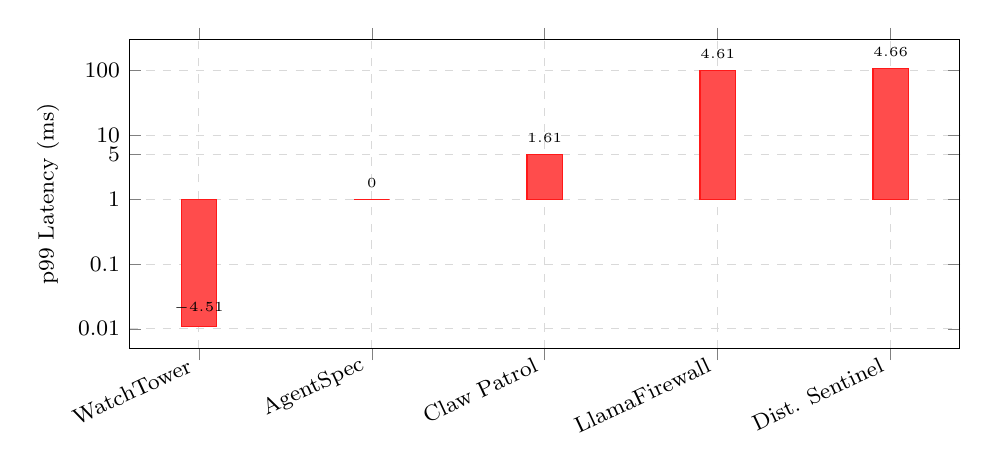
\begin{tikzpicture}
\begin{axis}[
  ybar,
  width=\columnwidth,
  height=5.5cm,
  bar width=0.45cm,
  symbolic x coords={WatchTower, AgentSpec, {Claw Patrol}, LlamaFirewall, {Dist. Sentinel}},
  xtick=data,
  x tick label style={font=\footnotesize, rotate=25, anchor=east},
  ylabel={p99 Latency (ms)},
  ylabel style={font=\footnotesize},
  ymode=log,
  ymin=0.005, ymax=300,
  ytick={0.01, 0.1, 1, 5, 10, 100},
  yticklabels={0.01, 0.1, 1, 5, 10, 100},
  tick label style={font=\footnotesize},
  grid=major,
  grid style={dashed, gray!30},
  nodes near coords,
  nodes near coords style={font=\tiny, anchor=south},
  every node near coord/.append style={yshift=1pt}
]
  \addplot[fill=red!70, draw=red!90] coordinates {
    (WatchTower, 0.011)
    (AgentSpec, 1)
    ({Claw Patrol}, 5)
    (LlamaFirewall, 100)
    ({Dist. Sentinel}, 106)
  };
\end{axis}
\end{tikzpicture}
\caption{p99 enforcement latency comparison (log scale). WatchTower achieves 0.011\,ms, a 9,636$\times$ improvement over the closest competitor (AgentSpec, 1\,ms). Note: LlamaFirewall and Distributed Sentinel latencies are from published papers~\cite{llamafirewall2025,sentinel2026}; AgentSpec and Claw Patrol latencies are reported as typical/target values.}
\label{fig:latency}
\end{figure}

% -------------------------------------------------------
\section{Discussion}
\label{sec:discuss}

\subsection{Why Determinism Beats LLM-in-the-Loop for Enforcement}
\label{sec:discuss:determinism}

A natural question is whether LLM classifiers (L7) should be on the hot path. Our evaluation argues against this. LLMs introduce three properties that are harmful for enforcement: non-determinism (same input, different verdict on different runs), latency variance (100--1,000\,ms), and prompt injection vulnerability (an attacker who knows the classifier prompt can craft inputs that evade it). Deterministic rule engines at L3 do not share these properties. The two-tier design in WatchTower places LLMs in the cold async path where their strengths (nuanced semantic understanding) are valuable and their weaknesses (latency, non-determinism) are tolerable.

\subsection{The Semantic Gap: Why Wire-Level Is Insufficient}
\label{sec:discuss:gap}

Claw Patrol~\cite{clawpatrol2026} achieves $<$5\,ms by operating at the wire level (HTTP/gRPC interception). This is excellent for blocking unknown tool types but cannot answer: ``Is this HTTP POST an exfiltration or a legitimate notification?'' The answer requires the call tree context --- specifically, whether the call appears in a data-retrieval workflow. WatchTower's enrichment layer (L2) provides exactly this context by reconstructing the AST and call tree. The semantic gap~\cite{observgap2026,archmatters2026} is structural; it cannot be closed by faster classifiers alone.

\subsection{Open Problems}
\label{sec:discuss:open}

\begin{enumerate}
  \item \textbf{Taint cleaning.} The current model has no mechanism for an agent to ``earn back'' trust through verified-clean behavior. A formal cleaning protocol is needed.

  \item \textbf{Multi-agent collusion.} The threat model assumes at most one compromised agent. BFT consensus at L6 provides partial protection but does not cover all collusion topologies.

  \item \textbf{Adaptive adversaries.} An attacker who observes enforcement decisions can calibrate attack parameters to stay below the quarantine threshold. Adaptive $\lambda$ and $\rho$ are needed.

  \item \textbf{Cross-organization taint.} When agents from multiple organizations share memory (e.g., via a federated MCP store), taint propagation crosses trust domain boundaries. Cross-domain taint protocols require federated identity infrastructure.

  \item \textbf{Policy expressiveness vs.\ completeness.} The YAML DSL supports common patterns but may not express all desired invariants. A formal policy language with a complete semantics is future work.

  \item \textbf{Scalability to large call trees.} The current AST enrichment is linear in call tree depth. For deep delegation chains, enrichment latency may grow non-trivially. A compressed representation (e.g., Bloom-filtered call tree hash) may be required.
\end{enumerate}

\subsection{Limitations}
\label{sec:discuss:limits}

WatchTower's interception requires integration with the agent runtime. Agents running in sandboxed environments with restricted introspection may not support the hermes hook pattern. The 0.011\,ms p99 latency is measured on a single machine; network-distributed agent clusters will add IPC latency. The 17-case corpus, while covering all three surfaces, is necessarily a sample; real-world attack diversity will be higher. Finally, the taint model's parameters ($\rho = 0.8$, $\lambda = 0.1\,\text{hr}^{-1}$, $Q = 0.7$) were calibrated against the MINJA corpus; different deployments may require recalibration.

% -------------------------------------------------------
\section{Conclusion}
\label{sec:conclusion}

We have presented WatchTower, an observation-first security framework for multi-agent AI systems that is the first published system to address all three attack surfaces --- prompt injection, capability abuse, and multi-agent contagion --- with cross-session taint tracking. The 9-layer architecture separates deterministic hot-path enforcement from expensive async analysis, achieving 0.011\,ms p99 latency while maintaining 100\% detection on a 17-case known-bad corpus. The formal taint propagation model enables detection of MINJA-class cross-session contagion attacks before the victim agent executes its next tool call --- a capability absent from all prior published systems. WatchTower is approximately 1,200 lines of Python 3.12 and is designed to integrate with existing agent frameworks via the hermes hook interface. We release the implementation, corpus, and evaluation tooling to support reproducibility.

% -------------------------------------------------------
\bibliographystyle{IEEEtran}
\bibliography{references}

\end{document}
